% ============================================================
%  SECTION 6 — PROJECT TIMELINE (Gantt chart)
% ============================================================

\begin{frame}{Project Timeline}
\centering
\scriptsize

\def\WeekStart{5}
\def\WeekEnd{15}
\def\numTasks{7}

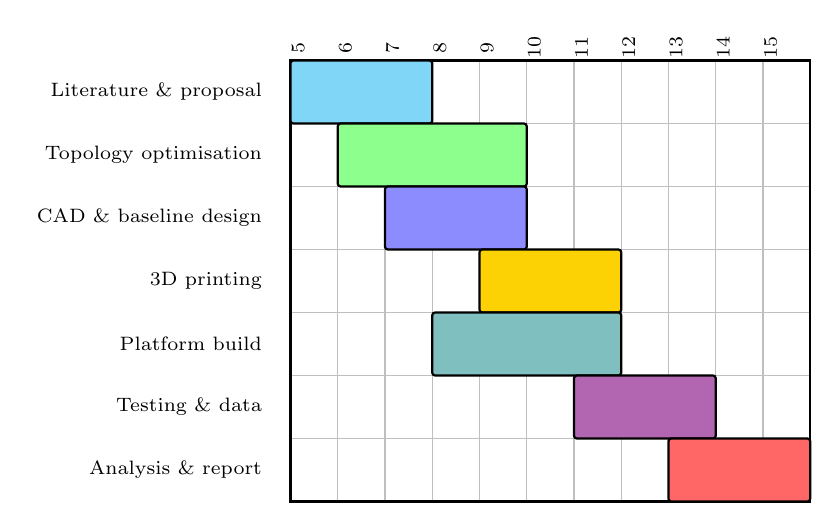
\begin{tikzpicture}[x=0.6cm, y=0.8cm]

  \tikzstyle{bar}     = [draw, rounded corners=1pt, thick]
  \tikzstyle{grid}    = [gray!50, thin]
  \tikzstyle{lbl}     = [anchor=east, align=right, font=\scriptsize]
  \tikzstyle{wlbl}    = [font=\scriptsize, anchor=south, rotate=90]

  \pgfmathtruncatemacro{\numCols}{\WeekEnd - \WeekStart + 1}
  \pgfmathtruncatemacro{\topRow}{\numTasks + 1}

  % ---- GRID ----
  \foreach \x in {0,...,\numCols}{
    \draw[grid] (\x,1) -- (\x,\topRow);
  }
  \foreach \y in {1,...,\numTasks}{
    \draw[grid] (0,\y) -- (\numCols,\y);
  }
  \draw[black,thick] (0,1) rectangle (\numCols,\topRow);

  % ---- WEEK LABELS ----
  \pgfmathtruncatemacro{\lastIdx}{\numCols-1}
  \foreach \idx in {0,...,\lastIdx}{
    \pgfmathtruncatemacro{\wnum}{\WeekStart+\idx}
    \node[wlbl] at (\idx+0.5,\topRow+0.2) {\wnum};
  }

  % ---- TASKS (top to bottom: row 7 down to row 1) ----

  % Row 7: Literature review & proposal
  \node[lbl] at (-0.4,7.5) {Literature \& proposal};
  \draw[bar,fill=cyan!50] (0,7) rectangle (3,8);       % wk 5--7

  % Row 6: Topology optimisation code
  \node[lbl] at (-0.4,6.5) {Topology optimisation};
  \draw[bar,fill=green!45] (1,6) rectangle (5,7);      % wk 6--9

  % Row 5: CAD modelling
  \node[lbl] at (-0.4,5.5) {CAD \& baseline design};
  \draw[bar,fill=blue!45] (2,5) rectangle (5,6);       % wk 7--9

  % Row 4: 3D printing
  \node[lbl] at (-0.4,4.5) {3D printing};
  \draw[bar,fill=yellow!70!orange] (4,4) rectangle (7,5); % wk 9--11

  % Row 3: Platform build & calibration
  \node[lbl] at (-0.4,3.5) {Platform build};
  \draw[bar,fill=teal!50] (3,3) rectangle (7,4);       % wk 8--11

  % Row 2: Testing & data collection
  \node[lbl] at (-0.4,2.5) {Testing \& data};
  \draw[bar,fill=violet!60] (6,2) rectangle (9,3);     % wk 11--13

  % Row 1: Analysis & report
  \node[lbl] at (-0.4,1.5) {Analysis \& report};
  \draw[bar,fill=red!60] (8,1) rectangle (11,2);       % wk 13--15

\end{tikzpicture}
\end{frame}
